% !TeX root = ../../../manual.tex
\chapter{Figures}

\section{Including Images}

The primary command for raster and vector image inclusion is
\verb|\includegraphics| from the \texttt{graphicx} package:

\begin{verbatim}
\includegraphics[width=\textwidth]{images/photo}
\includegraphics[height=5cm, keepaspectratio]{diagram}
\includegraphics[scale=0.5]{chart}
\end{verbatim}

\begin{longtblr}[
    caption = {Common \texttt{\textbackslash includegraphics} options},
    label = {tab:includegraphics-options},
]{colspec = {l l}, rowhead = 1}
    \toprule
    Option            & Effect \\
    \midrule
    width             & Scale to given width \\
    height            & Scale to given height \\
    scale             & Scale factor relative to natural size \\
    keepaspectratio   & Maintain aspect ratio when both width and height are set \\
    angle             & Rotate the image by the given angle in degrees \\
    trim              & Crop the image: \texttt{left bottom right top} \\
    clip              & Enable cropping set by \texttt{trim} \\
    draft             & Show a bounding box instead of the image \\
    page              & Select a page from a multi-page PDF \\
    \bottomrule
\end{longtblr}

OmniLaTeX configures \verb|\graphicspath| to search common asset directories.
Place images in \texttt{images/}, \texttt{figures/}, or \texttt{assets/}
without specifying the subdirectory in the path argument.

\section{SVG Graphics}

OmniLaTeX supports SVG graphics through the \texttt{svg} package, which
converts SVG files to PDF using Inkscape at compile time.

\begin{verbatim}
\includesvg[width=\textwidth]{logo}
\end{verbatim}

\begin{itemize}
    \item \textbf{Requirements:} Inkscape must be installed and the
          \texttt{-{}-shell-escape} flag must be passed to the \LaTeX{}
          engine.
    \item \textbf{Search paths:} Configure additional SVG search directories
          with \verb|\svgpath|:
\begin{verbatim}
\svgpath{{images/svg/}{assets/vector/}}
\end{verbatim}
    \item \textbf{Debugging:} Use \verb|\debugtikzsvg| to enable verbose
          output during SVG conversion, showing Inkscape commands and
          intermediate file paths.
\end{itemize}

Converted PDFs are cached next to the source SVG file. Delete the cached
\texttt{.pdf} to force re-conversion after editing the SVG.

\section{Text Over Images}

When placing text over images with varying backgrounds, use contour commands
for legibility:

\begin{verbatim}
% White contour for dark backgrounds
\ctrw{Readable on dark images}

% Black contour for light backgrounds
\ctrb{Readable on light images}
\end{verbatim}

These commands wrap the \texttt{contour} package to draw a thin outline around
each glyph, ensuring the text remains legible regardless of the underlying
image content.

\section{TikZ Basics}

OmniLaTeX loads common TikZ libraries through
\texttt{omnilatex-tikz-core.sty}. The following libraries are available by
default:

\begin{verbatim}
\usetikzlibrary{
    positioning,
    arrows.meta,
    calc,
    shapes.geometric,
    decorations.pathreplacing,
    backgrounds,
    fit,
}
\end{verbatim}

\begin{verbatim}
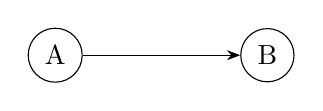
\begin{tikzpicture}
    \node[draw, circle] (a) {A};
    \node[draw, circle, right=2cm of a] (b) {B};
    \draw[-{Stealth}] (a) -- (b);
\end{tikzpicture}
\end{verbatim}

Coordinate systems, basic shapes, nodes, and edges all follow standard TikZ
conventions. Refer to the TikZ manual for the full set of available options.

\section{Subfigures}

Use the \texttt{subcaption} package for side-by-side figures with individual
labels:

\begin{verbatim}
\begin{figure}[htbp]
    \centering
    \begin{subfigure}[b]{0.45\textwidth}
        \centering
        \includegraphics[width=\textwidth]{img-left}
        \caption{Left subfigure}
        \label{fig:sub-left}
    \end{subfigure}
    \hfill
    \begin{subfigure}[b]{0.45\textwidth}
        \centering
        \includegraphics[width=\textwidth]{img-right}
        \caption{Right subfigure}
        \label{fig:sub-right}
    \end{subfigure}
    \caption{Two subfigures side by side.}
    \label{fig:subfigures}
\end{figure}
\end{verbatim}

Subfigure labels are formatted as \emph{(a)}, \emph{(b)}, etc. Cross-reference
individual subfigures with \verb|\cref{fig:sub-left}| and the parent figure
with \verb|\cref{fig:subfigures}|.

\section{Figure References}

Use the \texttt{cleveref} package for automatic naming of figure references:

\begin{verbatim}
As shown in \cref{fig:example}, ...
See also \cref{fig:sub-left,fig:sub-right}.
\end{verbatim}

OmniLaTeX configures the \texttt{cleveref} capitalization names so that
\verb|\Cref| produces \emph{Figure} at the start of a sentence. Customize
the naming with \verb|\crefname|:

\begin{verbatim}
\crefname{figure}{fig.}{Figs.}
\Crefname{figure}{Figure}{Figures}
\end{verbatim}
